
	\begin{enumerate}
	\item Дата собрания: 15.10.14
	\item Цель:
		\begin{itemize}
		\item Заменить омни-колеса на обычные
		\item Начать готовить профили для подъемника
		\item Решить проблему с барабаном
		\end{itemize}
	\item Результаты:
		\begin{itemize}
		\item Было установлено два колеса, оба ведущие. Так как теперь они установлены не в углах конструкции уменьшилась площадь опорной поверхности $\Rightarrow$ уменьшилась стабильность робота.
		\item Профили были распилены на отдельные части определенного размера и пропилены отверстия для креплений
		\item Проблема не была решена, вся конструкция ходит туда-сюда по-прежнему. Было решено оставить этот элемент в покое на данный момент времени и заняться колесной базой.
		\end{itemize}
	\item Идеи и планы:
		\begin{itemize}
		\item Установить оставшиеся колеса и испытать робота на поле
		\item Начать строить подъемник
		\end{itemize}
		\begin{figure} [h]
			\centering
			\begin{minipage}{0.3\linewidth}
				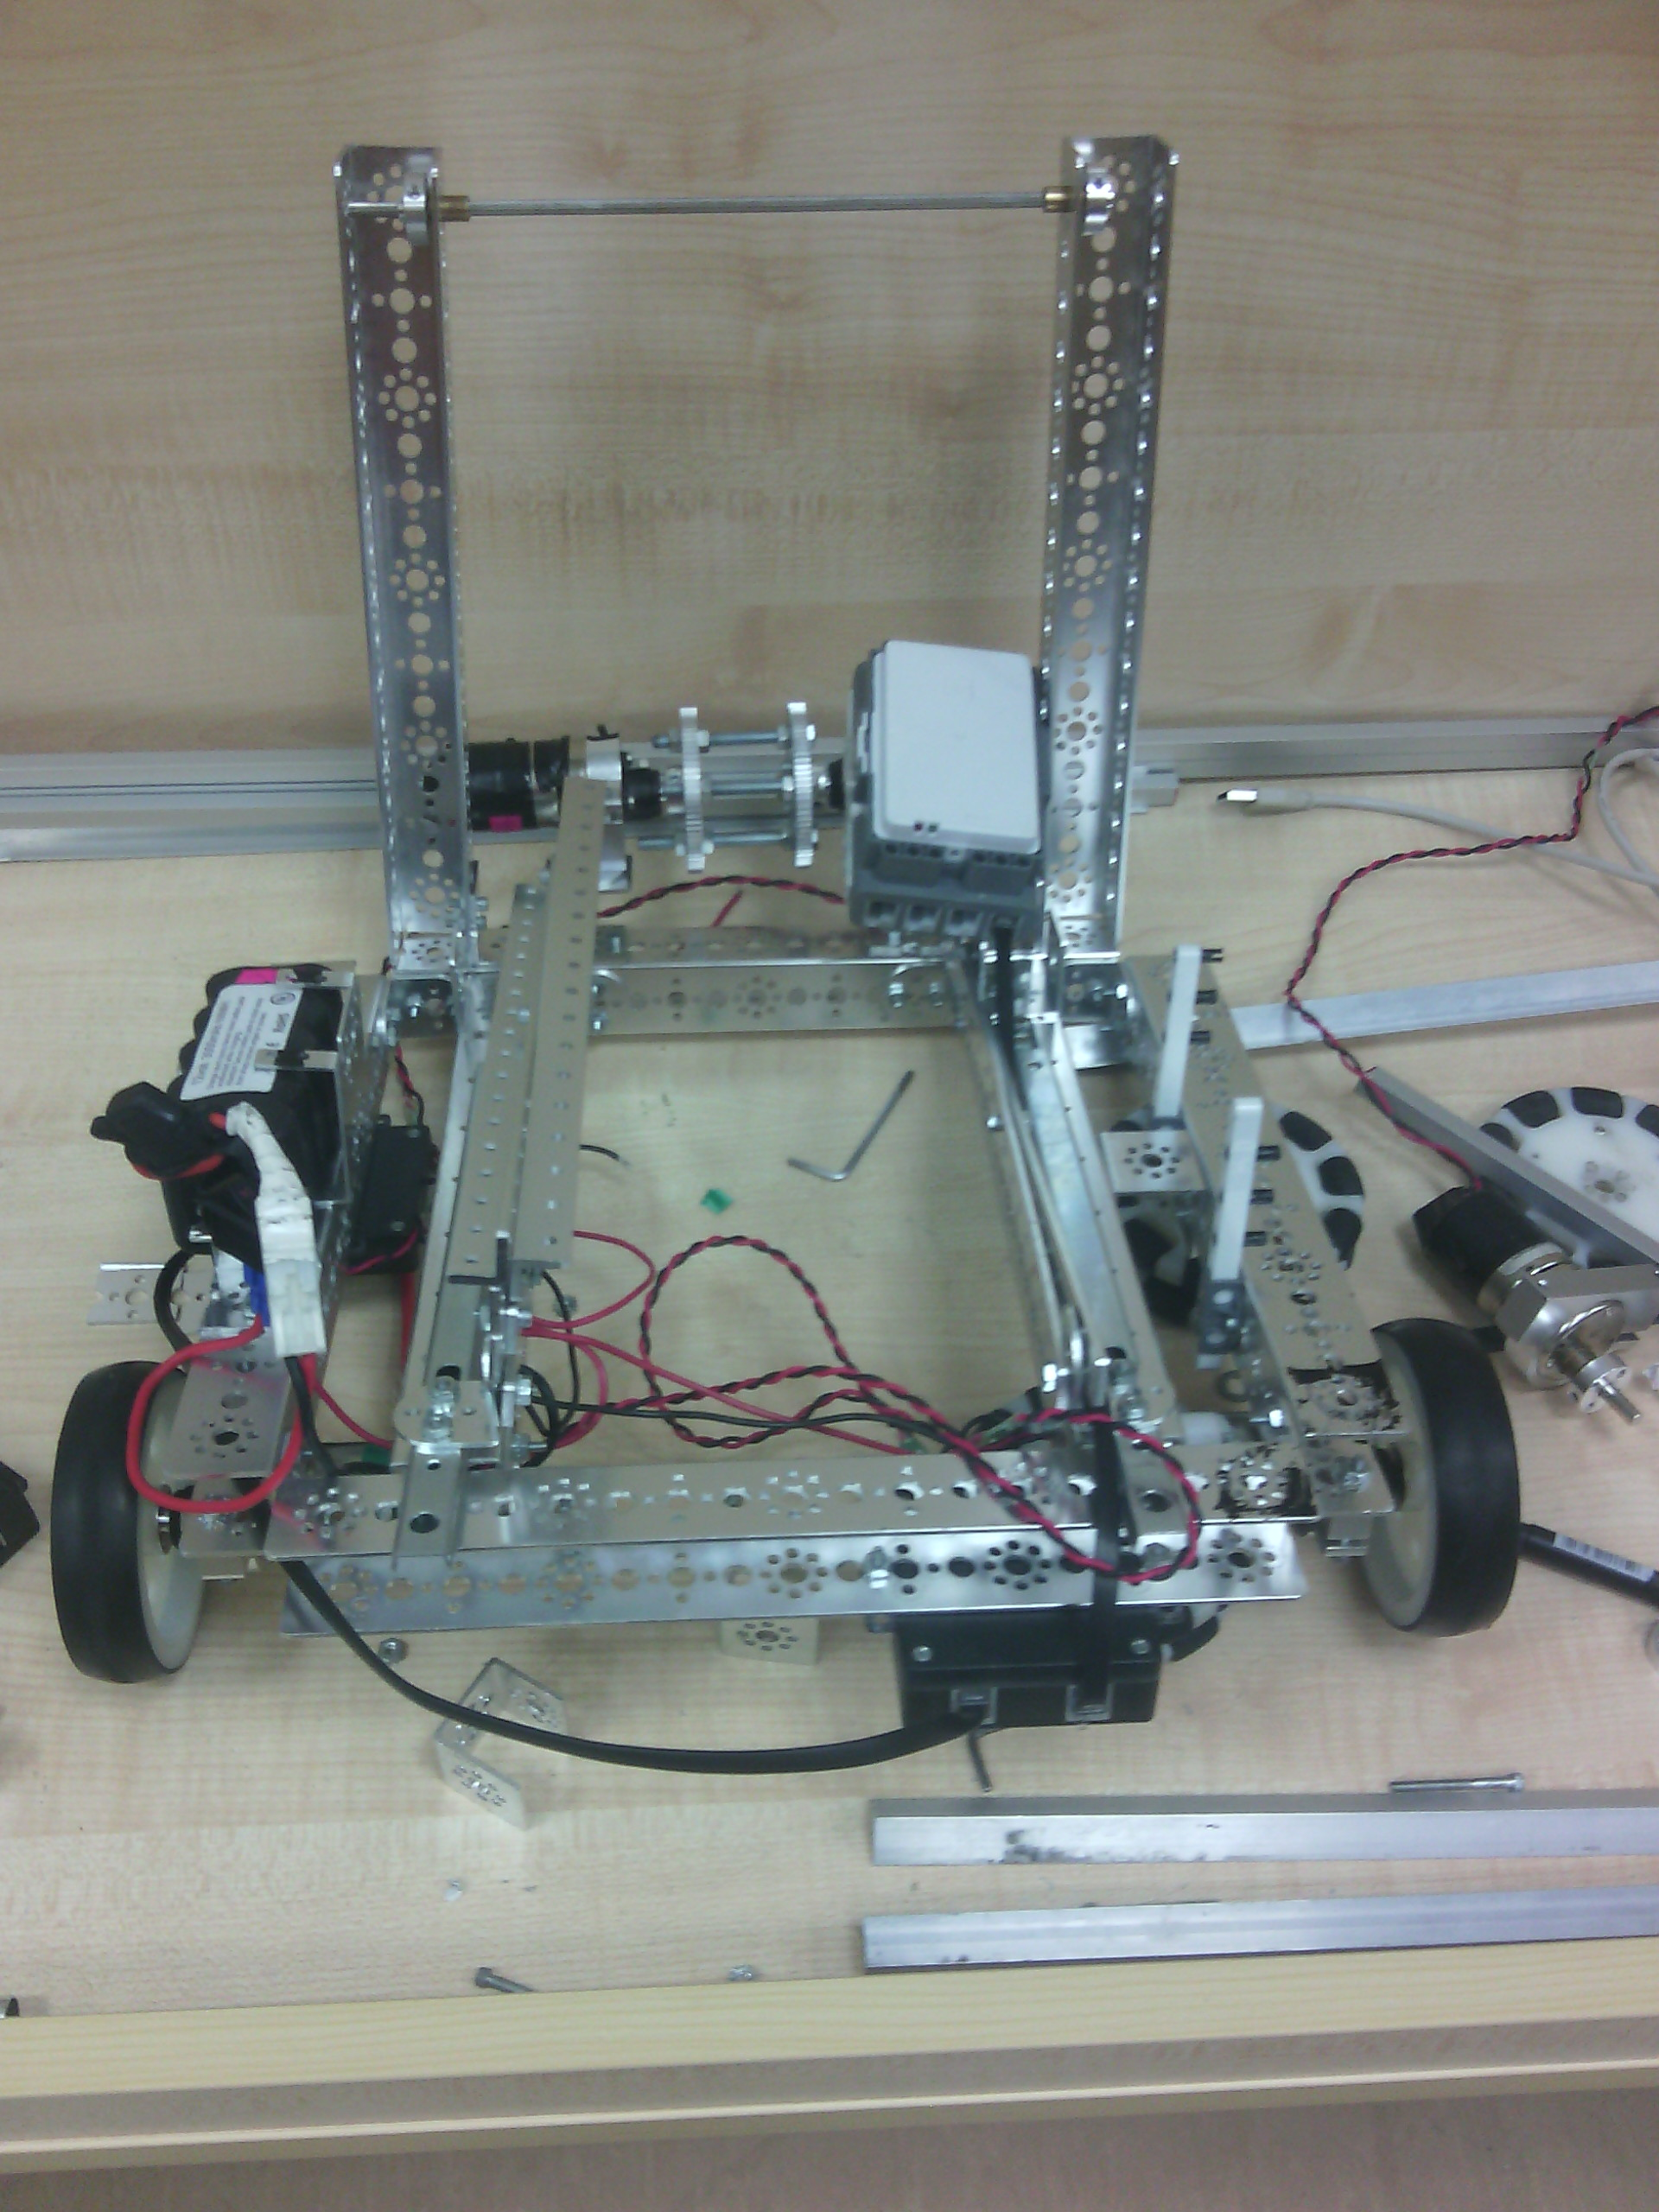
\includegraphics[width=35mm,height=35mm]{Days/15.10.14/8_1_robot}\\ Рисунок 8
			\end{minipage}
		\end{figure}
	\end{enumerate}
\fillpage
\newpage

